%%%%%%%%%%%%%%%%%%%%%%%%%%%%%%%%%%%%%%%%%%%%%%%%
% E.Pinault-Bigeard - e.pinault-bigeard@upsti.fr
% http://s2i.pinault-bigeard.com
% CC BY-NC-SA 2.0 FR - http://creativecommons.org/licenses/by-nc-sa/2.0/fr/
%%%%%%%%%%%%%%%%%%%%%%%%%%%%%%%%%%%%%%%%%%%%%%%%
\documentclass[11pt]{article}
%%%%%%%%%%%%%%%%%%%%%%%%%%%%%%%%%%%%%%%%%%%%%%%%
% Package UPSTI_Document
%%%%%%%%%%%%%%%%%%%%%%%%%%%%%%%%%%%%%%%%%%%%%%%%

\usepackage{import}
%
%%%%%%%%%%%%%%%%%%%%%%%%%%%%%%%%%%%%%%%%%%%%%%%%
% Package UPSTI_Document
%%%%%%%%%%%%%%%%%%%%%%%%%%%%%%%%%%%%%%%%%%%%%%%%
\usepackage{subcaption}
\usepackage[usenames, svgnames, dvipsnames]{xcolor}
\usepackage{UPSTI_Document}
\usepackage{pgfplots}
\usepackage{import}
\definecolor{darkspringgreen}{rgb}{0.09, 0.45, 0.27}

\newcommandx*{\dessinRepereFigGeo}[5][1=\vx{},2=\vy{},3=\vz{},4=,5=0]
	{
		\draw [->,very thick] (0,0) -- (1,0) ;
		\draw [->,very thick] (0,0) -- (0,1) ;
    \fill[white] (0,0) circle (0.13);
    \draw [->,very thick] (0,0) circle (0.13);
    \ifnumequal{#5}{0} {% z vers nous
      \fill[black] (0,0) circle (0.03);
      \draw [->,thick] (0,0) circle (0.04);
    }{% z vers la feuille
  		\begin{scope} [rotate=45]
  			\draw [-,thick] (0,-0.12) -- (0,0.12) ;
  			\draw [-,thick] (-0.12,0) -- (0.12,0) ;
  		\end{scope}
    }
		\draw [anchor=north west] (1.1,0) node {${#1}$};
		\draw [anchor=south west] (0,1.1) node {${#2}$};
		\draw [anchor=north east] (-0.1,0) node {${#3}$};
		\draw [anchor=north west] (-0.1,-0.1) node {${#4}$};
	}

	\usepackage{array}
	\newcolumntype{L}[1]{>{\raggedright\let\newline\\\arraybackslash\hspace{0pt}}m{#1}}
	\newcolumntype{C}[1]{>{\centering\let\newline\\\arraybackslash\hspace{0pt}}m{#1}}
	\newcolumntype{R}[1]{>{\raggedleft\let\newline\\\arraybackslash\hspace{0pt}}m{#1}}

	\usepackage{pifont}% http://ctan.org/pkg/pifont
\newcommand{\cmark}{\color{green}\ding{51}}%
\newcommand{\xmark}{\color{red}\ding{55}}%
\newcommand{\fmark}{\ding{229}}%
\newcommand{\itemc}{\item[\cmark]}%
\newcommand{\itemx}{\item[\xmark]}%
\newcommand{\itemf}{\item[\fmark]}%

\usepackage{tikz-timing}
\usepackage{circuitikz}
\usepackage{pdfpages}
%---------------------------------%
% Paramètres du package
%---------------------------------%

% Version du document (pour la compilation)
% 1: Document prof
% 2: Document élève
% 3: Document à publier
\newcommand{\UPSTIidVersionDocument}{2}

% Classe
% 1: PTSI				6: PSI*			11: TSI2		16: Spé
% 2: PT	(par défaut)	7: MPSI			12: ATS
% 3: PT*				8: MP			13: PC
% 4: PCSI				9: MP*			14: PC*
% 5: PSI				10: TSI1		15: Sup
%\newcommand{\UPSTIidClasse}{2}



% Matière
% 1: S2I (par défaut)    2: IPT     3: TIPE
% 6: Vie au lycée
\newcommand{\UPSTIvariante}{5}
\newcommand{\UPSTIidMatiere}{0}
\newcommand{\UPSTIintituleMatiere}{Automatique}
\newcommand{\UPSTIsigleMatiere}{Autom}
% Type de document
% 0: Custom*				7: Fiche Métho de			14: Document Réponses
% 1: Cours (par défaut)		8: Fiche Synthèse    		15: Programme de colle
% 2: TD     				9: Formulaire
% 3: TP						10: Memo
% 4: Colle					11: Dossier Technique
% 5: DS						12: Dossier Ressource
% 6: DM						13: Concours Blanc
% * Si on met la valeur 0, il faut décommenter la ligne suivante:
%\newcommand{\UPSTItypeDocument}{Custom}
\newcommand{\UPSTIidTypeDocument}{1}

% Titre dans l'en-tête


% Titre dans l'en-tête

\newcommand{\UPSTIvariante}{5}

\newcommand{\UPSTItitreEnTete}{Automatisme industriel}
%\newcommand{\UPSTItitreEnTetePages}{}
\newcommand{\UPSTIsousTitreEnTete}{Introduction aux API}


% Titre
%\newcommand{\UPSTItitrePreambule}{Automatisme industriel}
\newcommand{\UPSTItitre}{La programmation d'un Automate Industriel}

% Durée de l'activité (pour DS, DM et TP)
\newcommand{\UPSTIduree}{3h30}

% Note de bas de première page
%\newcommand{\UPSTInoteBasDePremierePage}{Geoffrey Vaquette}
% Numéro (ajoute " n°1" après DS ou DM)
\newcommand{\UPSTInumero}{2}

% Numéro chapitre
%\newcommand{\UPSTInumeroChapitre}{1}

% En-tête customisé
%\newcommand{\UPSTIenTetePrincipalCustom}{UPSTIenTetePrincipalCustom}

% Message sous le titre
%\newcommand{\UPSTImessage}{Message sous le titre}


% Référence au programme
%\newcommand{\UPSTIprogramme}{\EPBComp \EPBCompP{B1-02}, \EPBCompP{B2-49}, \EPBCompS{B2-50}, \EPBCompS{B2-51}, \EPBCompP{C1-07}, \EPBCompP{C1-08}}

% Si l'auteur n'est pas l'auteur par défaut
%\renewcommand{\UPSTIauteur}{WWOOOOOOWW}

% Si le document est réalisé au nom de l'équipe
%\newcommand{\UPSTIdocumentCollegial}{1}

% Source
\newcommand{\UPSTIsource}{G. Vaquette}

% Version du document
\newcommand{\UPSTInumeroVersion}{1.0}

%-----------------------------------------------
\UPSTIcompileVars		% "Compile" les variables
%%%%%%%%%%%%%%%%%%%%%%%%%%%%%%%%%%%%%%%%%%%%%%%%


% Titre
%\newcommand{\UPSTItitrePreambule}{Automatisme industriel}
\newcommand{\UPSTItitre}{Exercice de synthèse} 
\usetikzlibrary{arrows,automata,circuits.plc.ladder}

\newlength{\ladderskip}
\setlength{\ladderskip}{5\tikzcircuitssizeunit} % 5\tikzcircuitssizeunit = 35pt
\newlength{\ladderrungsep}
\setlength{\ladderrungsep}{.2\ladderskip}
\def\ladderrungend#1{\pgftransformyshift{-#1\ladderskip-\ladderrungsep}}

\ctikzset{
	logic ports=ieee,
	logic ports/scale=0.7,
}



\newcommand{\automaintienMachineEtat}[0]{
\begin{tikzpicture}[->,>=stealth',shorten >=1pt,auto,node distance=3cm,
                    semithick]
  %\tikzstyle{every state}=[fill=none,draw=none,text=white]

  \node[initial,state] (A)              {M1};
  \node[state]         (B) [right of=A] {M2};

  \path (A) edge [bend left]  node {$B_pM$} (B)
        (B) edge [bend left]  node {$B_pA$} (A);
\end{tikzpicture}
}


%%%%%%%%%%%%%%%%%%%%%%%%%%%%%%%%%%%%%%%%%%%%%%%%
% Début du document
%%%%%%%%%%%%%%%%%%%%%%%%%%%%%%%%%%%%%%%%%%%%%%%%
\begin{document}
\UPSTIbuildPage

%\UPSTIobjectif{Durant cette activité, nous allons analyser une trame pour l'envoi d'informations sur une étiquette.}

%\tableofcontents
%\pagebreak


\section{Introduction}
Cette séance de synthèse avant la semaine de TP test a pour objectif de revoir et d'appliquer les notions vues jusqu'ici. Elle portera sur un système d'ascenseur que nous utiliserons durant les TPs du semestre prochain. 

\begin{figure}[ht]
	\centering
	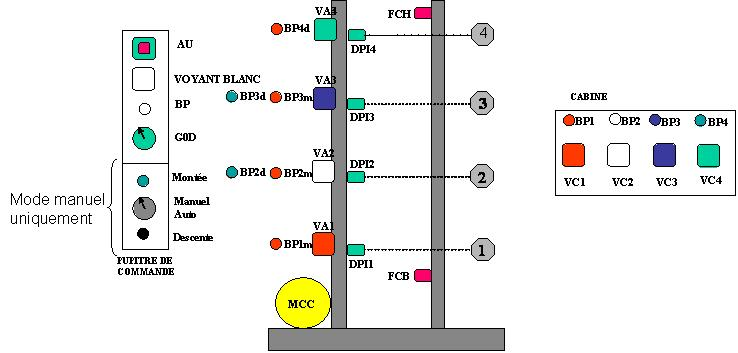
\includegraphics[width=.85\linewidth]{images/ascenseur.jpg}
	\caption{Partie opérative de l'ascenseur}
	\label{fig:schemaPartieOperative}
\end{figure}

Le système est composé d'une cabine se déplaçant dans une gaine d'ascenseur ainsi que de boutons et voyants à chaque étage (Figure~\ref{fig:schemaPartieOperative}).

L’ascenseur dessert quatre étages. La cabine est actionnée par un moteur à courant continu MCC.
La commande du moteur comporte une alimentation et un inverseur de sens de rotation à relais.

Chaque étage est muni d’un détecteur de présence inductif (DPI1, DPI2, DPI3, DPI4) et d’un
voyant d’appel (VOY1, VOY2, VOY3, VOY4).
Chaque palier dispose d'un ou deux bouton poussoir d’appel pour (BP1m, BP2m, BP2d, BP3m, BP3d et BP4d)
La cabine est munie de 4 boutons d’appel : (BP1, BP2, BP3, BP4)
Le pupitre de commande comporte un coup de point d’urgence (AU) normalement fermé, un commutateur 3 positions
gauche/auto/droite. En position « auto », deux détecteurs mécaniques de fin de course FCB et
FCH coupent l’alimentation du moteur en cas de dépassement des positions limites. 
%Si la cabine est bloquée en haut ou en bas, on court-circuite le FCH en position gauche et le FCB en position « manu ». On a alors accès à la commande du variateur et on peut ainsi débloquer la cabine.

Le moteur électrique est actionné via un variateur de vitesse commandé en tension 0-10V. 

\section{Travail à faire}
\begin{UPSTIactivite}
	\UPSTIquestion{Faire la liste des capteurs du système}

	\UPSTIquestion{En déduire le nombre d'entrées logiques, numériques et analogiques}

	\UPSTIquestion{Faire la liste des actionneurs du système}

	\UPSTIquestion{En déduire le nombre de sorties logiques, numériques et analogiques}

	\UPSTIquestion{Combien de modules supplémentaires faudra-t-il installer sur le LOGO pour commander cet ascenseur ?}

\end{UPSTIactivite}

\begin{UPSTIactivite}
	On suppose ici que l'on utilise une automate LOGO pour effectuer la commande de cet ascenseur. 
	\UPSTIquestion{Dessiner le cablage des boutons interieur de la cabine}
	\UPSTIquestion{Dessiner le câblage des capteurs inductif de présence cabine}
	\UPSTIquestion{Dessiner le câblage des voyants d'étage à l'aide de sortie à relais}
	\UPSTIquestion{Dessiner le câblage du voyant blanc à l'aide d'une sortie à transistor}
\end{UPSTIactivite}

\begin{UPSTIactivite}
	Un programme met en sécurité l'ascenseur lorsqu'il atteint les capteurs fin de course situés tout en haut ou tout en bas de la colonne ou lorsque le bouton d'arrêt d'urgence est pressé. Un mémento M1 est à 1 lorsque le système peut fonctionner. 
	\UPSTIquestion{Programmer le programme de sécurité de l'ascenseur}
\end{UPSTIactivite}


\begin{UPSTIactivite}
	A l'aide de deux relais 2 positions que vous commanderez à l'aide d'une sortie à transistor : 
	\UPSTIquestion{Dessiner un câblage permettant de changer le sens de rotation du moteur à courant continu}
	\UPSTIquestion{A l'aide d'une sortie relais supplémentaire, ajouter la possibilité d'arrêter le moteur}
\end{UPSTIactivite}

\end{document}
